\Transcb{yellow}{blue}{The Muppets on Ice}
\twocolumn
\begin{center}
{\blue Tue 09-aug-2011 07:23:18 UTC}\\
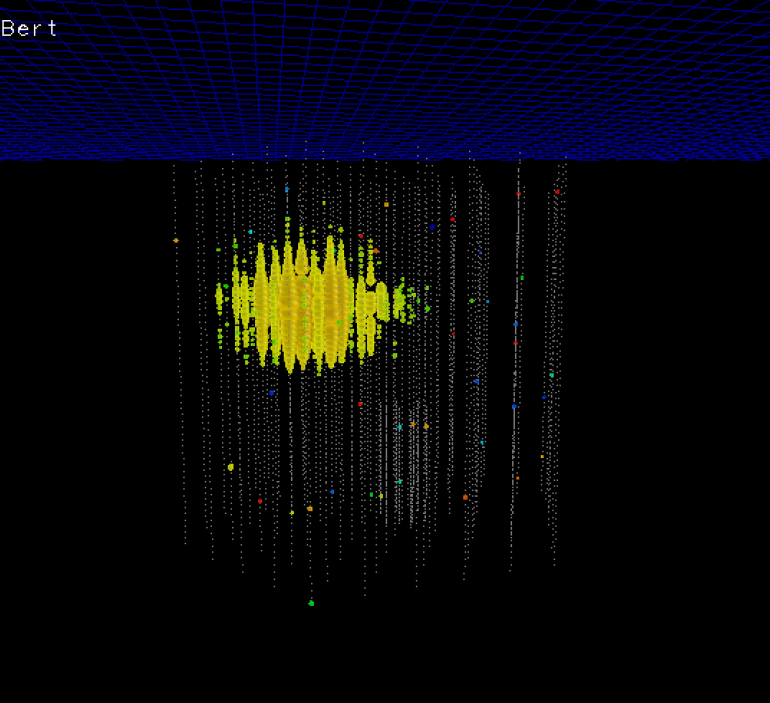
\includegraphics[keepaspectratio,width=13cm]{bert}\\
$1.04 \pm 0.16$ PeV
\end{center}
{\blue Atmosferische $\nu$ achtergrond ?}

\newpage

\begin{center}
{\blue Tue 03-jan-2012 03:34:01 UTC}\\
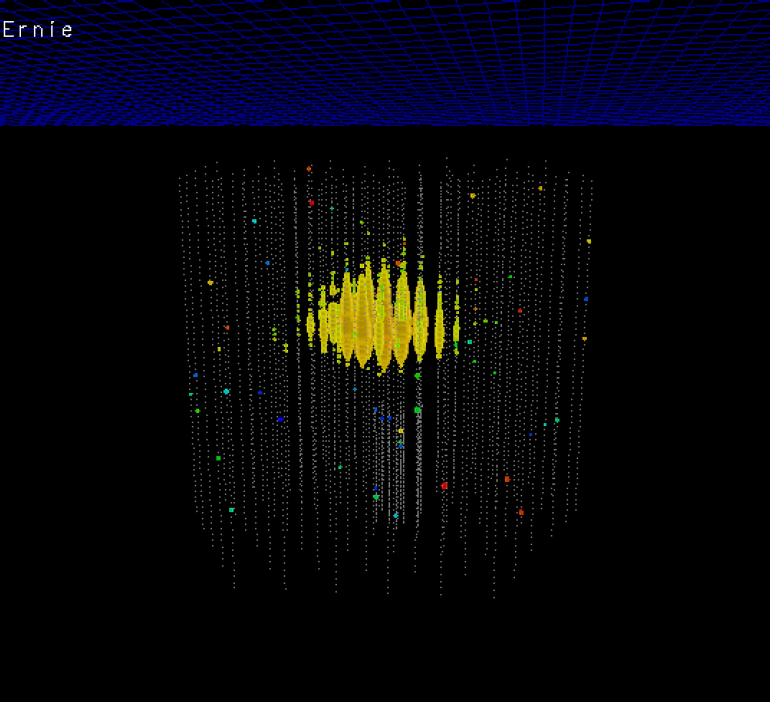
\includegraphics[keepaspectratio,width=13cm]{ernie}\\
$1.14 \pm 0.17$ PeV
\end{center}
{\blue Slechts ca. 0.3\% kans op achtergrond}

\Tr
\twocolumn[\begin{center}{\blue Nog een aantal additionele events gevonden}\end{center}]
%
\begin{center}
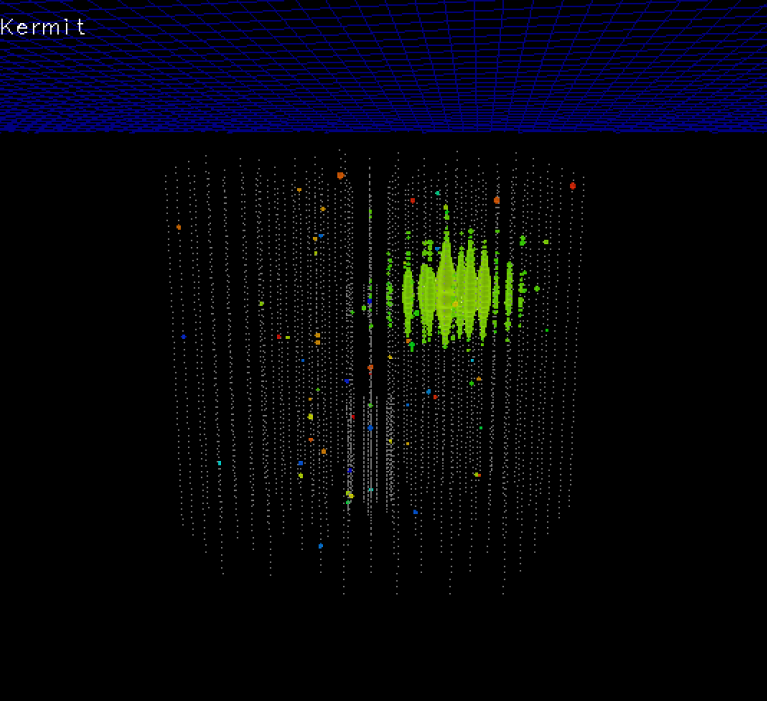
\includegraphics[keepaspectratio,width=13cm]{kermit}
\end{center}

\newpage

\begin{center}
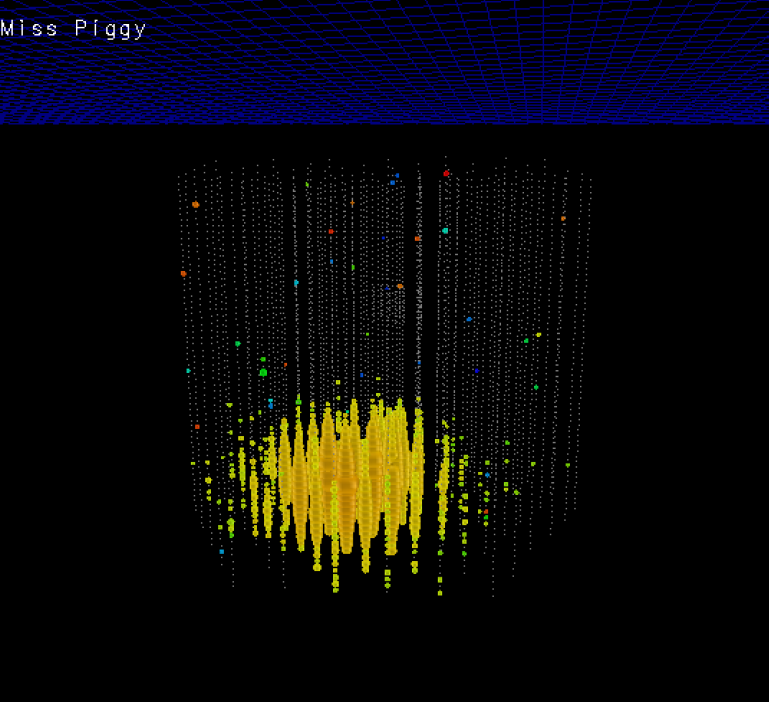
\includegraphics[keepaspectratio,width=13cm]{miss-piggy}
\end{center}

\Tr
\twocolumn[\begin{center}{\blue Ook enkele $\mu$ spoorsignaturen}\end{center}]
%
\begin{center}
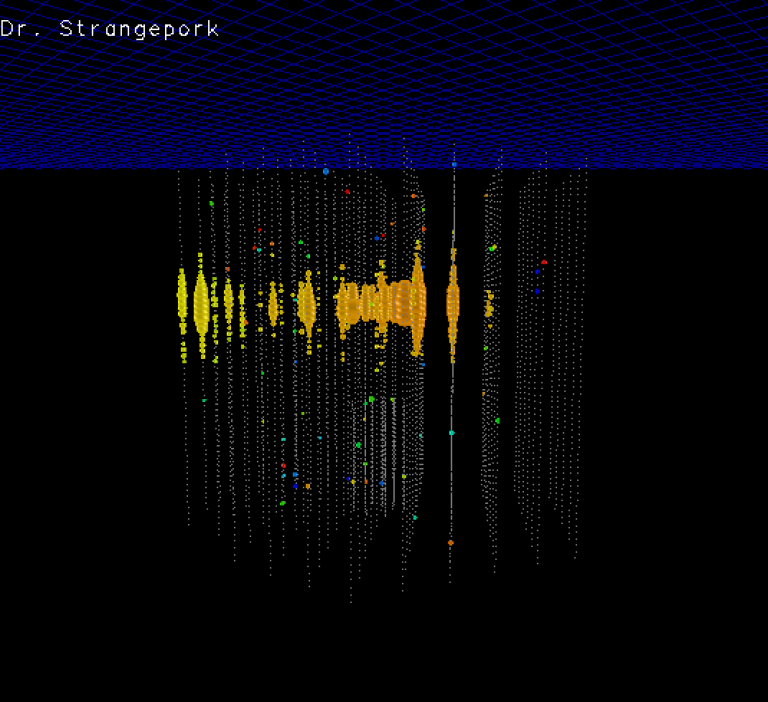
\includegraphics[keepaspectratio,width=13cm]{dr-strangepork}
\end{center}

\newpage

\begin{center}
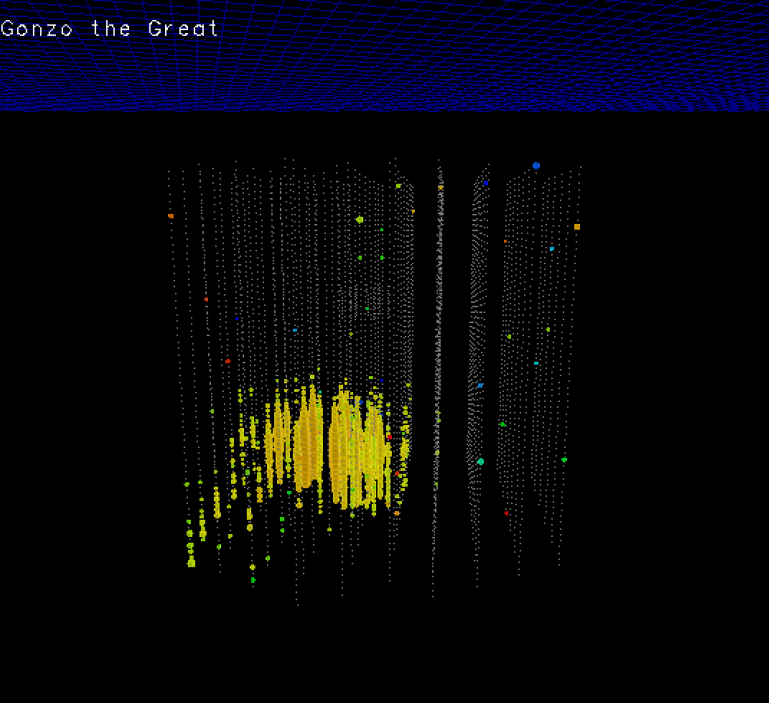
\includegraphics[keepaspectratio,width=13cm]{gonzo-the-great}
\end{center}

\Tr
\onecolumn
\begin{center}
{\blue Karakteristieken van 82 events}
\end{center}
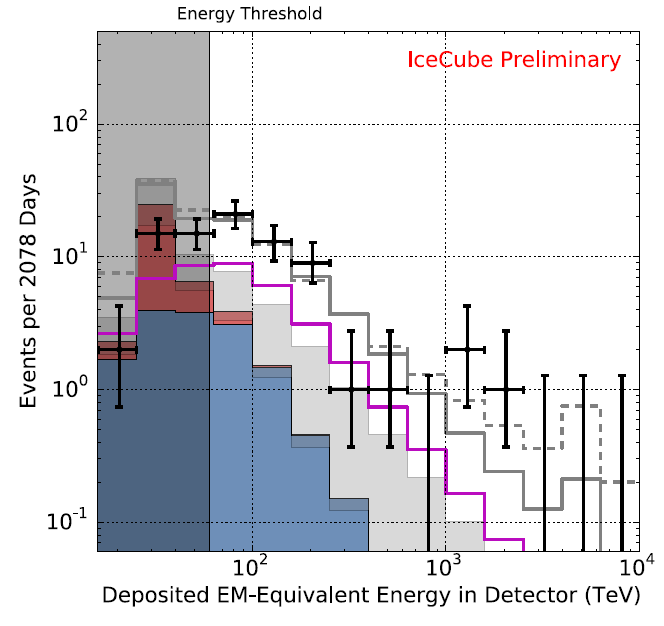
\includegraphics[keepaspectratio,height=11cm]{hese-e-6yr}
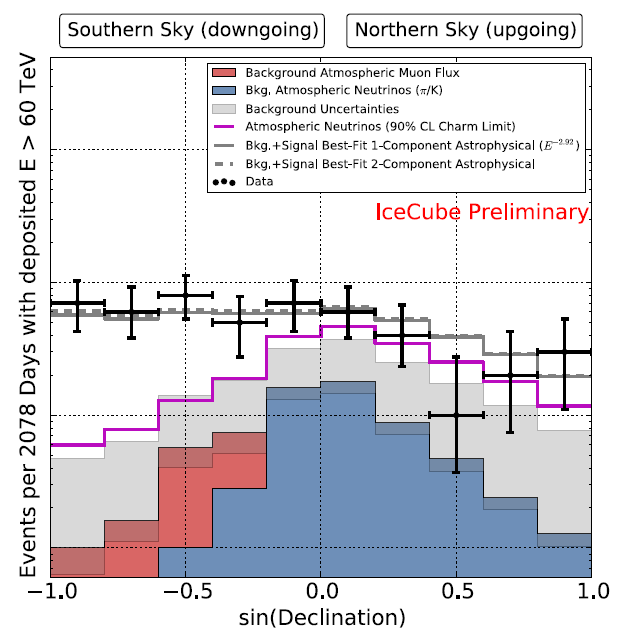
\includegraphics[keepaspectratio,height=11cm]{hese-decl-6yr}
\begin{center}
\colorbox{yellow}{Aanduiding voor kosmische hoog-energetische neutrino's}
\end{center}

\Tr
\onecolumn
\begin{center}
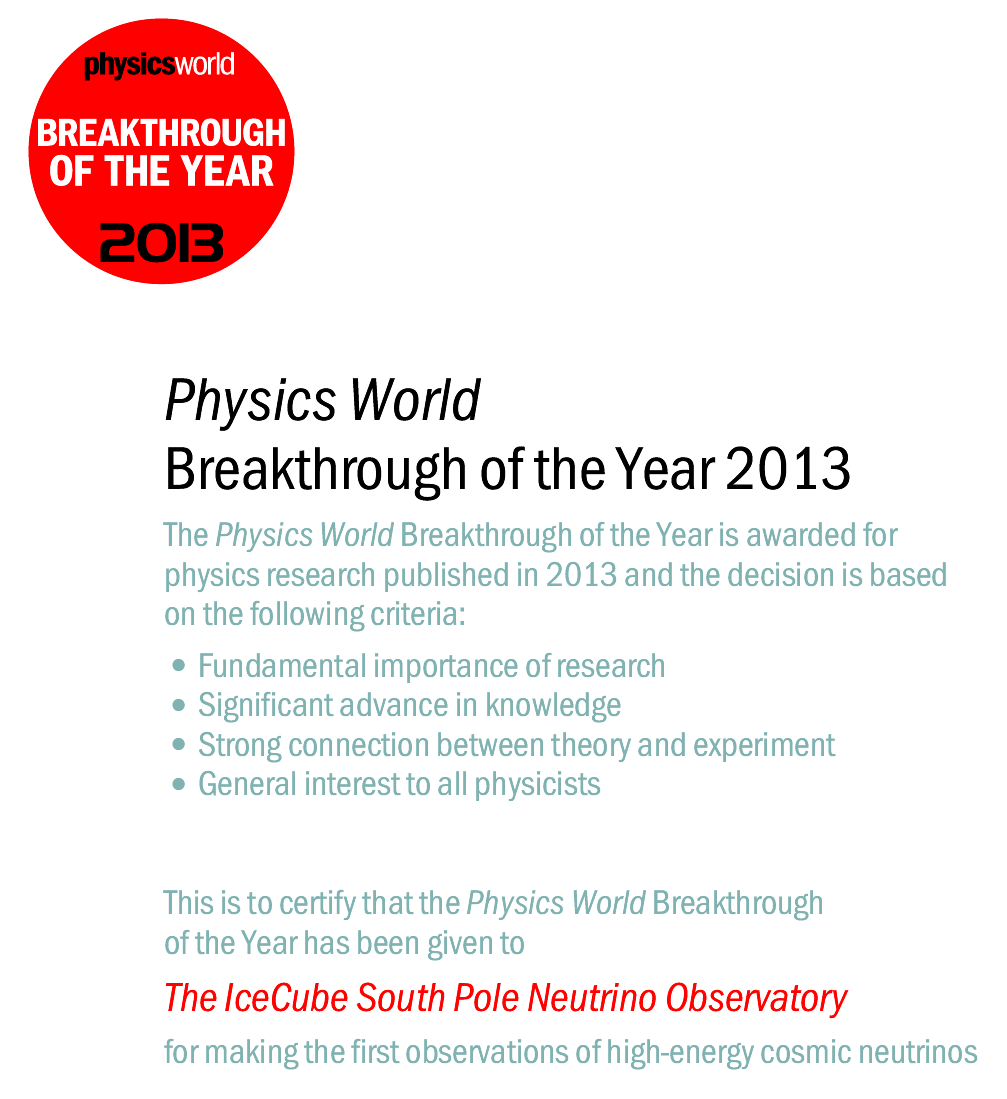
\includegraphics[keepaspectratio,height=15cm]{breakthrough}\\
\end{center}

\Tr
\onecolumn
\begin{center}
{\blue Herkomst van deze 82 events}\\[5mm]
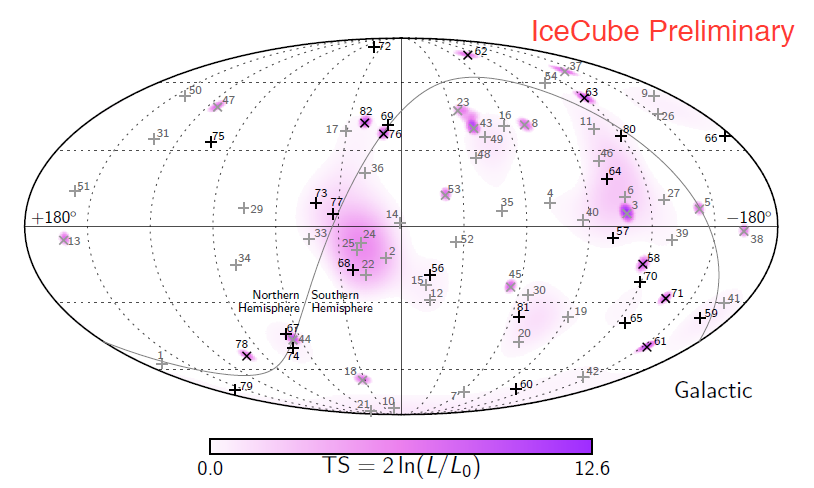
\includegraphics[keepaspectratio,height=13cm]{hese-skymap-gal-6yr}\\
\colorbox{yellow}{Geen bewijs voor puntbron(nen)}
\end{center}
